\documentclass[aspectratio=43, xcolor=table]{beamer}
\usepackage{../../preamble_math}
\usepackage{subcaption}
\usepackage{booktabs}

%%%%%% Logo definitions %%%%%%
\def\logoconference{} % no conference logo
% logo path / logo height / logo yshift
\def\institutionlogos{ICL_Logo_Blue_CMYK.pdf/0.4cm/0.3cm,boeing.pdf/0.85cm/0cm}
\def\separation{0.7cm}
\def\titletopskip{0.6cm} % space above the title on the title page
%%%%%%%%%%%%%%%%%%%%%%%%%%%%%%

%%%%%% Custom colors %%%%%%
\definecolor{customcolor}{RGB}{3, 75, 152}
\definecolor{mplgreen}{RGB}{44, 160, 44}  % matplotlib tab:green / tab:orange
\definecolor{mplorange}{RGB}{255, 127, 14}
%%%%%%%%%%%%%%%%%%%%%%%%%%%

%%%%%% Load custom styling %%%%%%
\usepackage{../../myImperialBeamerTemplate}
\usetikzlibrary{arrows.meta, calc}
% Overlay-aware TikZ: \begin{scope}[visible on=<2->] keeps the space when hidden
\tikzset{
	invisible/.style={opacity=0},
	visible on/.style={alt={#1{}{invisible}}},
	alt/.code args={<#1>#2#3}{\alt<#1>{\pgfkeysalso{#2}}{\pgfkeysalso{#3}}},
}
%%%%%%%%%%%%%%%%%%%%%%%%%%%%%%

%%%%%%% Metadata %%%%%%%
\title{Transition over surface gaps in laminar boundary layers}
\author{
	\texorpdfstring{\underline{Víctor Ballester Ribó}$^1$, Jeffrey Crouch$^2$, \\
	Yongyun Hwang$^1$, Spencer Sherwin$^1$}{Víctor Ballester Ribó, Jeffrey Crouch, Yongyun Hwang, Spencer Sherwin}
}
\institute{
  $^1$Department of Aeronautics, Imperial College London, UK \\
  $^2$The Boeing Company, USA
}
\date{Boeing Farnborough, 21 October 2026}
%%%%%%%%%%%%%%%%%%%%%%%%%%

\newcommand\dstar{{\delta^*}}
\newcommand{\refnote}[1]{\vfill{\fontsize{6}{7}\selectfont\textit{#1}\par}}
\newcommand{\takeaway}[1]{%
	\begin{beamercolorbox}[rounded=true, shadow=false, sep=0.15cm]{block body}
		\small #1
	\end{beamercolorbox}}
\setbeamercolor{block body}{bg=customcolor!10}
% same box as \takeaway, in grey
\newcommand{\graybox}[1]{%
	\begin{beamercolorbox}[rounded=true, shadow=false, sep=0.15cm]{gray box}
		\small #1
	\end{beamercolorbox}}
\setbeamercolor{gray box}{bg=gray!15}

% Coordinates on 3d2dStabilityCurveRe1000.pdf as fractions of the image:
% x = (314.5 + w*433/130)/1063, y = (64 + 81.25*d)/397

% Small copy of the 2D/3D stability map in the top-right corner;
% \stabmap[<width>]{<file>} swaps in another map, e.g. one highlighting a region
\newcommand{\stabmap}[2][3.0cm]{%
	\begin{tikzpicture}[remember picture, overlay]
		\node[anchor=north east, inner sep=0pt] (stabmap) at ([xshift=-0.05cm, yshift=-0.05cm]current page.north east)
		{\includegraphics[width=#1]{Images/#2}};
	\end{tikzpicture}}

% Slide counter (bottom right), hidden on the title slide
\setbeamertemplate{footline}{%
	\ifnum\insertframenumber>1
		\hfill{\fontsize{7}{8}\selectfont\color{gray}\insertframenumber/\inserttotalframenumber}\hspace{0.3cm}\vspace{0.2cm}%
	\fi}

\begin{document}

\begin{frame}\titlepage\end{frame}

%======================================================================
\begin{frame}{About me}
	\begin{itemize}
		\setlength\itemsep{0.6em}
		\item \textbf{BSc Mathematics}, Autonomous University of Barcelona (2019--2023)
		      \begin{itemize}
			      \item Thesis: numerical propagation of Earth-orbiting spacecraft trajectories.
		      \end{itemize}
		\item \textbf{MSc Applied \& Theoretical Mathematics}, Dauphine--PSL, Paris (2023--2024)
		      \begin{itemize}
			      \item Started interest in computational fluid dynamics.
			      \item Thesis: spreading of 2D turbulence (ENS Paris).
		      \end{itemize}
		\item \textbf{PhD in Aeronautics}, Imperial College London (2024--present)
		      \begin{itemize}
			      \item Funded by \textbf{The Boeing Company}.
			      \item Supervisors: Spencer Sherwin and Yongyun Hwang; collaboration with Jeff Crouch.
		      \end{itemize}
	\end{itemize}
\end{frame}

%======================================================================
\begin{frame}{Outline}
	\setbeamercovered{transparent=25}
	\begin{columns}[c]
		\begin{column}{0.5\linewidth}
			\small
			\begin{enumerate}
				\setlength\itemsep{0.6em}
				\item<1> Motivation: surface gaps and the experiments of Crouch \emph{et al.} (2022)
				\item<2> Numerical framework
				\item<3> Global stability analysis: 2D and 3D stability boundaries
				\item<4> Two-dimensional dynamics: TS-wave amplification ($\Delta n$)
				\item<5> Three-dimensional dynamics and transition
				\item<6> Compressibility: Mach-number effects
				\item<7> Conclusions and outlook
			\end{enumerate}
		\end{column}
		\begin{column}{0.48\linewidth}
			\begin{overlayarea}{\linewidth}{6cm}
				\vfill
				\centering
				\only<1>{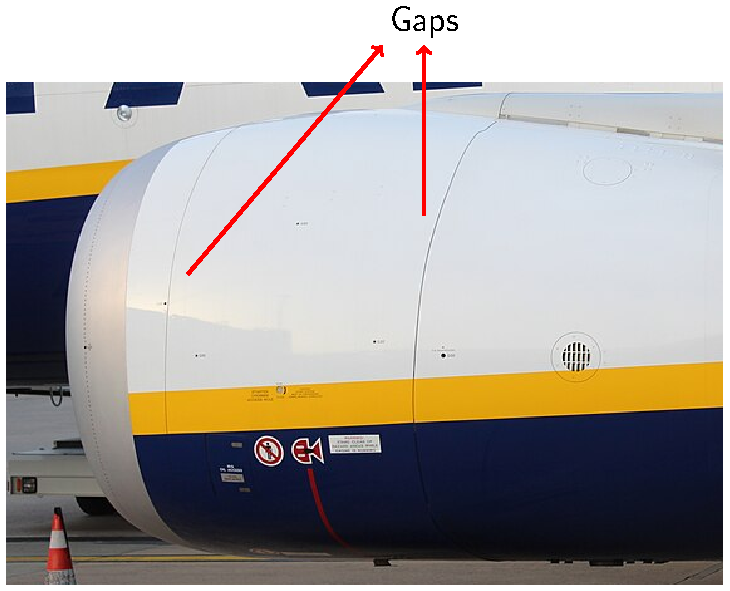
\includegraphics[width=\linewidth]{Images/nacelle.pdf}}%
				\only<2>{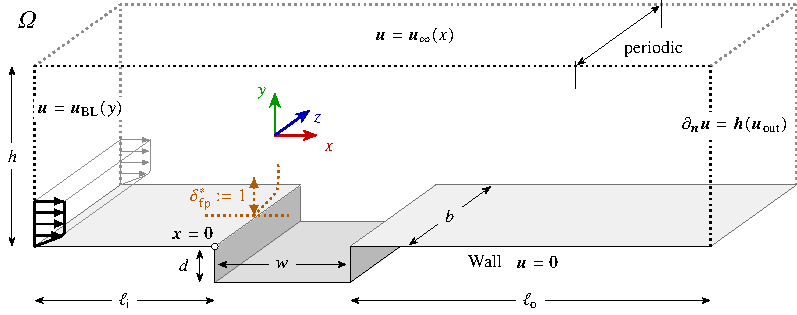
\includegraphics[width=\linewidth]{Images/domainBaseflow3D.pdf}}%
				\only<3>{}%
				\only<4>{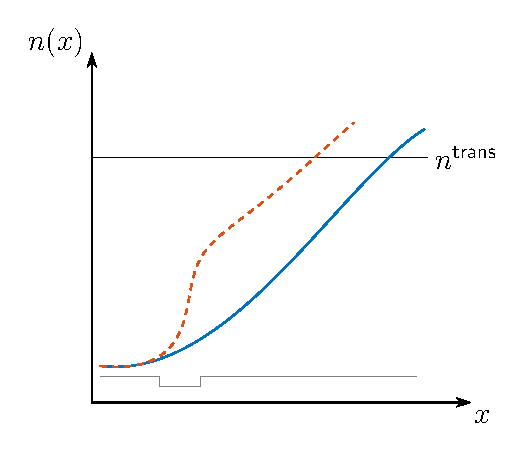
\includegraphics[width=\linewidth]{Images/amplificationQualititiveNfactorCurves.pdf}}%
				\only<5>{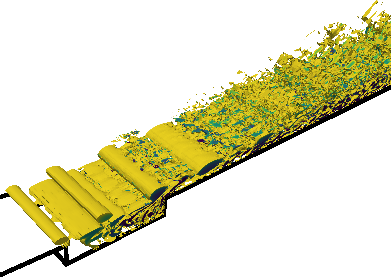
\includegraphics[width=\linewidth]{Images/trans_d4w19_3d_L2crit_17_big.pdf}}%
				\only<6>{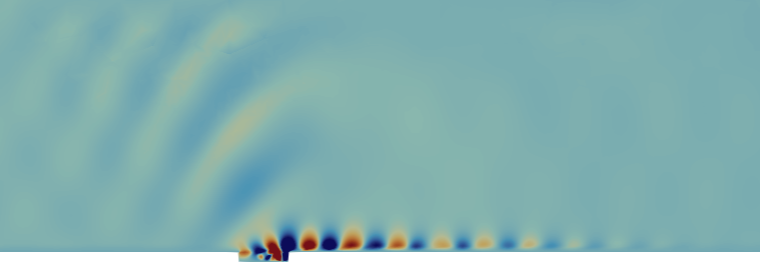
\includegraphics[width=\linewidth]{Images/d3w15Ma0.6_gapZoom.png}}%
				\vfill
			\end{overlayarea}
		\end{column}
	\end{columns}
\end{frame}

%======================================================================
\section{Motivation}
\begin{frame}{Why surface gaps?}
	\begin{itemize}
		\item Laminar flow $\Rightarrow$ lower skin friction $\Rightarrow$ lower fuel burn.
	\end{itemize}
	\begin{columns}[c, onlytextwidth]
		\begin{column}{0.45\linewidth}
			\begin{itemize}
				\item Real surfaces have imperfections that leave \textbf{steps and gaps}.
				\item<2-> Near the leading edge $\dstar\sim O(0.1\,\mathrm{mm})$, so a millimetre gap spans several $\dstar$.
				\item<2-> Tighter tolerances are expensive.
			\end{itemize}
			\vspace{0.3cm}
			\uncover<3->{\takeaway{The question is not \emph{whether} gaps can be removed but \emph{how large} one may be before it matters.}}
		\end{column}
		\hfill
		\begin{column}{0.5\linewidth}
			\begin{figure}
				\centering
				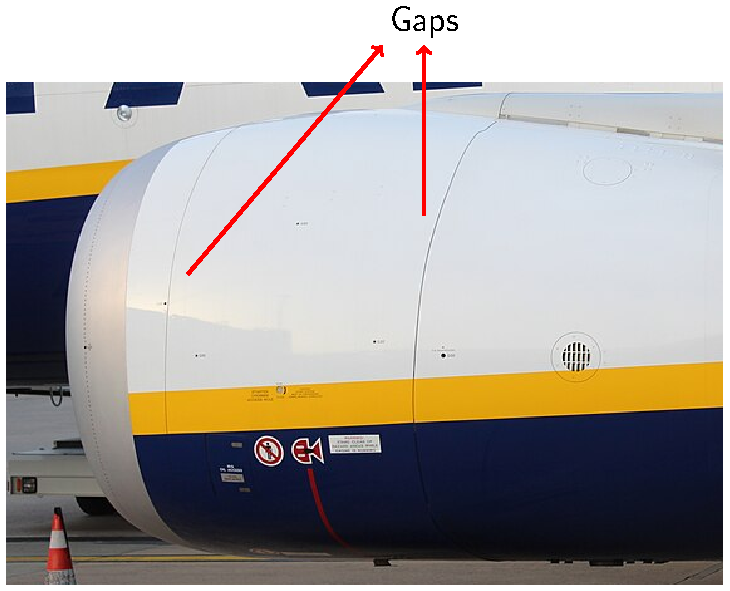
\includegraphics[width=\linewidth]{Images/nacelle.pdf}
				\caption{Engine nacelle of a Boeing 737.}
			\end{figure}
		\end{column}
	\end{columns}
\end{frame}

\begin{frame}{The $e^N$ method}
	\begin{itemize}
		\item In quiet flight conditions:\\
		      \begin{center}
			      receptivity $\longrightarrow$ TS-wave growth $\longrightarrow$ breakdown
		      \end{center}\pause
	\end{itemize}
	\begin{columns}[c, onlytextwidth]
		\begin{column}{0.499\linewidth}
			\begin{itemize}
				\setlength\itemsep{0.5em}

				\item Linear growth of a mode:
				      $$ n(x) = \log\frac{A(x)}{A_0} = \int_{x_0}^{x} -\alpha_i \,\dd{s}. $$\pause
				\item Transition is correlated with a threshold $n=N$.\pause
				\item \textbf{Variable-$N$ approach} for imperfections: $N = N_0 - \Delta N$.
			\end{itemize}
		\end{column}
		\begin{column}{0.48\linewidth}
			\begin{figure}
				\centering
				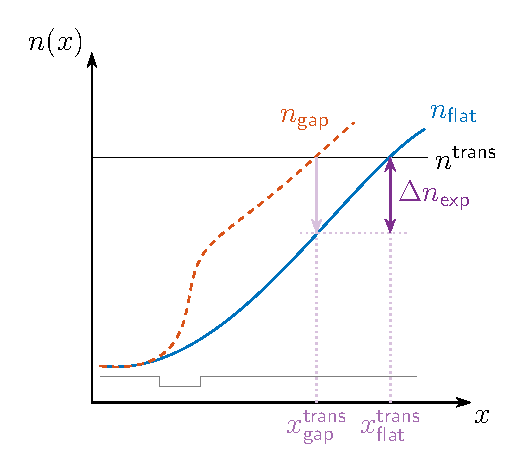
\includegraphics[width=\linewidth]{Images/amplificationQualititiveNfactorOnlyExpLabels.pdf}
			\end{figure}
		\end{column}
	\end{columns}
	\refnote{Smith \& Gamberoni (1956); van Ingen (1956); Crouch, Kosorygin \& Ng (2006); Crouch (2021).}
\end{frame}

\begin{frame}{Crouch \emph{et al.} (2022): experimental set-up}
	\begin{columns}[c]
		\begin{column}{0.48\linewidth}
			\begin{itemize}
				\setlength\itemsep{0.4em}
				\item Airfoil-like $C_p$.
				\item $M<0.1$, $Tu\approx0.03\%$.
				\item Spanwise-uniform rectangular gaps (length based on $\dstar$ at the upstream edge of the gap):
				      $$0<w<110,$$ $$0<d<11.$$\pause
				\item Transition length $\xi = \dfrac{x_\text{T,gap} - x_\text{gap}}{x_{\text{T,flat}}-x_\text{gap}}$.
			\end{itemize}
		\end{column}\hspace{-1.0cm}
		\begin{column}{0.5\linewidth}
			\begin{figure}
				\centering
				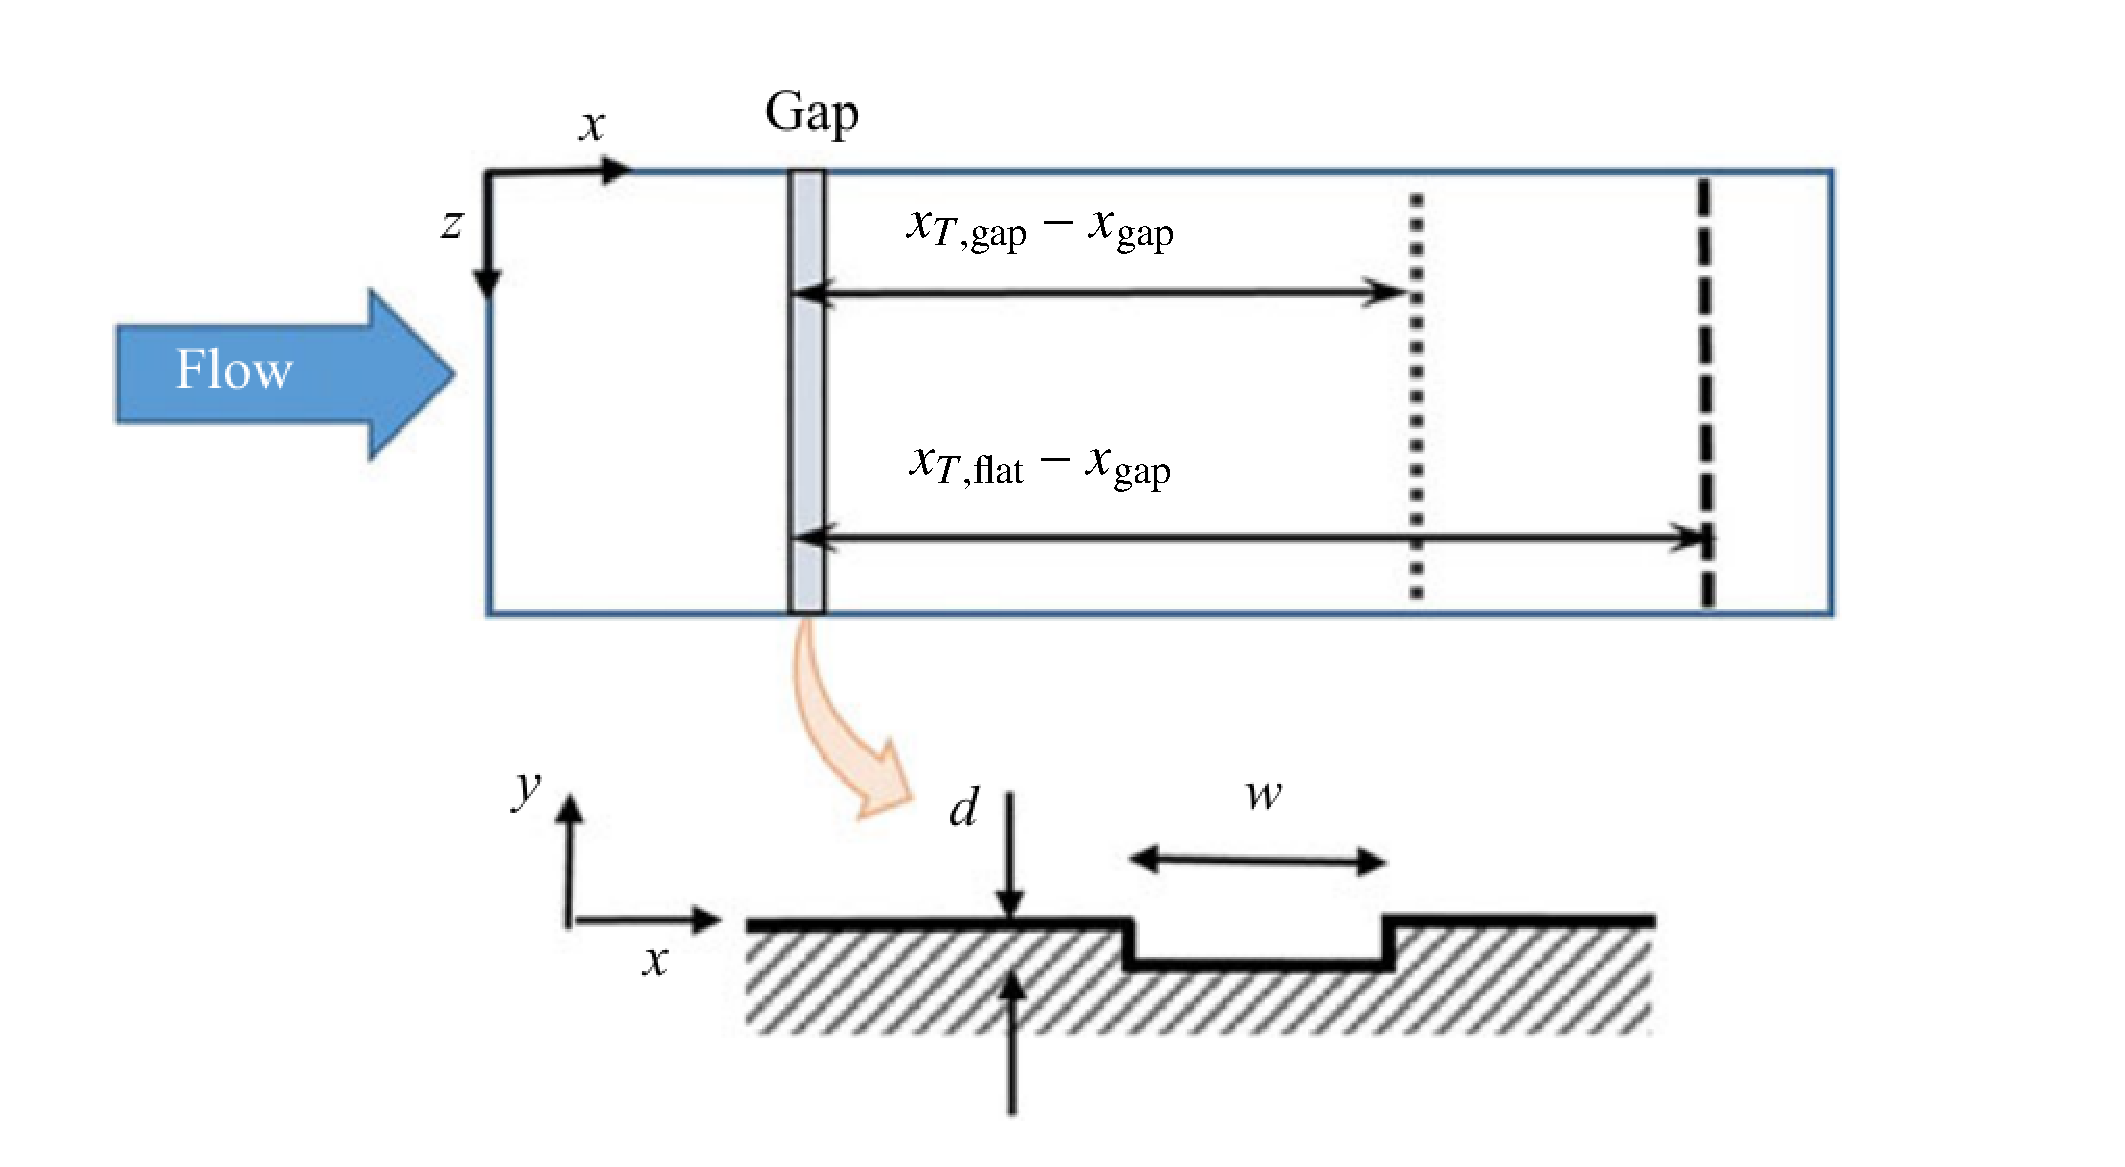
\includegraphics[width=1.2\linewidth]{Images/jeffSetupRelabelled.pdf}
			\end{figure}
		\end{column}
	\end{columns}
	\refnote{Crouch JD, Kosorygin VS, Sutanto MI, Miller GD. Characterizing surface-gap effects on boundary-layer transition dominated by Tollmien--Schlichting instability. Flow. 2022;2:E8.}
\end{frame}

\begin{frame}{Distribution of $\xi$}
	\begin{figure}
		\centering
		% left panel alone first, then with the zoomed panel (same size, so no jump)
		\includegraphics<1>[width=\linewidth]{Images/jeffScatterLeft.pdf}%
		\includegraphics<2->[width=\linewidth]{Images/jeffScatterZoom.pdf}
	\end{figure}
	\begin{itemize}
		\item Most gaps move transition only moderately ({\boldmath$\xi>50\%$}).
		\item Beyond $w\gtrsim20$ and $d\gtrsim2$: transition jumps to the gap (\textcolor{red}{\boldmath$\xi<10\%$}).
	\end{itemize}
	\uncover<3->{\takeaway{Why does transition move upstream? The gap \textbf{amplifies the TS waves}, so they reach breakdown earlier: $N_0\to N_0-\Delta N$.}}
\end{frame}

\begin{frame}{From $\xi$ to $\Delta N$: two limiting behaviours}
	\begin{itemize}
		\item Shift in transition $\Rightarrow$ extra TS amplification: $\Delta N = n_\text{flat}(x_\text{T,flat}) - n_\text{flat}(x_\text{T,gap})$.\pause
		\item Grey band: transition at the gap (\textcolor{red}{$\xi<10\%$}).
	\end{itemize}
	\begin{columns}[c]
		\begin{column}{0.61\linewidth}
			\begin{figure}
				\centering
				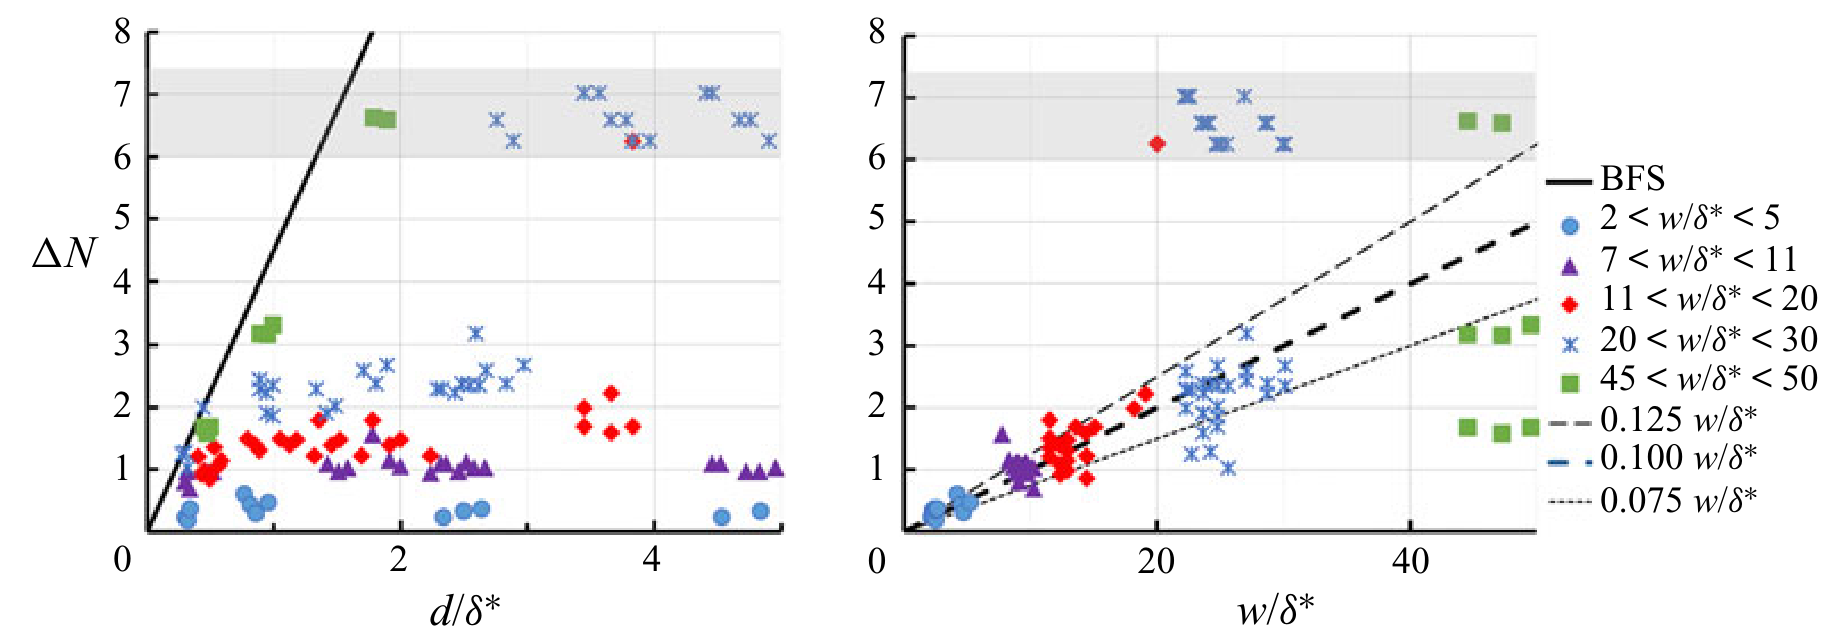
\includegraphics[width=\linewidth]{Images/jeffDeltaNClean.png}
			\end{figure}
		\end{column}
		\begin{column}{0.38\linewidth}
			\begin{figure}
				\centering
				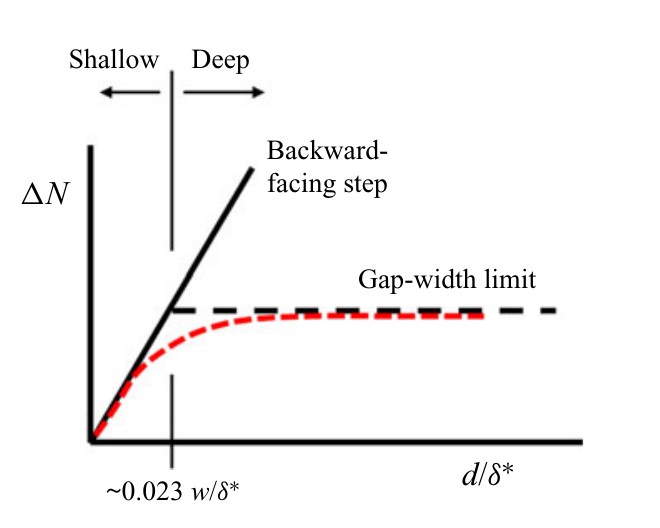
\includegraphics[width=\linewidth]{Images/jeffSchematic.png}
			\end{figure}
		\end{column}
	\end{columns}
	\vspace{0.2cm}
	\pause
	\small
	$$
		\Delta N \approx
		\begin{cases}
			4.4\, d & d/w \lesssim 0.023 \quad\text{(shallow: like a BFS)}   \\
			0.1\, w & d/w \gtrsim 0.023 \quad\text{(deep: set by the width)}
		\end{cases}
	$$
	\vspace{-0.2cm}
	$$
		\text{Smooth fit:}\quad\Delta N \approx 0.1w\tanh\left(\frac{44d}{w}\right)
	$$
\end{frame}

\begin{frame}{Fitted $\Delta N$ contours in the $(w,d)$ plane}
	\begin{figure}
		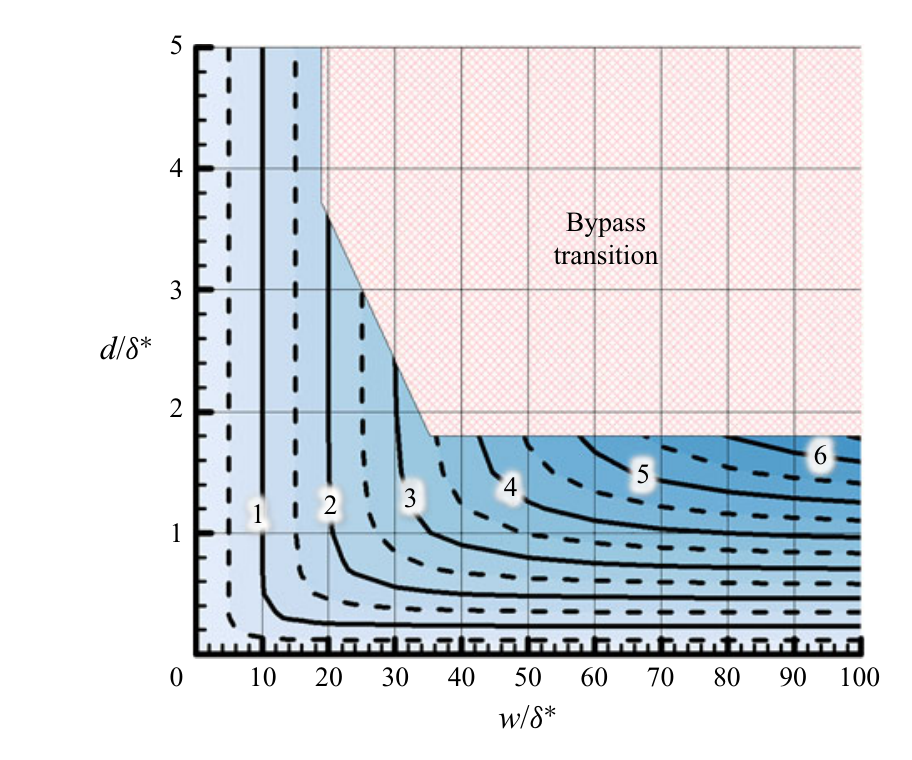
\includegraphics[height=0.85\textheight]{Images/jeffContours.png}
	\end{figure}
\end{frame}

\begin{frame}{Open questions}
	\textbf{Questions addressed in this talk:}
	\begin{enumerate}
		\setlength\itemsep{0.8em}
		\item What sets the \textbf{shape} of the $\Delta N$ curves, and how does it depend on $\Rey$ and $\mathrm{Ma}$?\pause
		\item What \textbf{mechanism} is behind the ``bypass transition''?\\
		      {\small Linear instability $\neq$ transition. Which instabilities are needed?}
	\end{enumerate}
\end{frame}

%======================================================================
\section{Numerical framework}
\begin{frame}{Numerical set-up}
	\begin{figure}
		\centering
		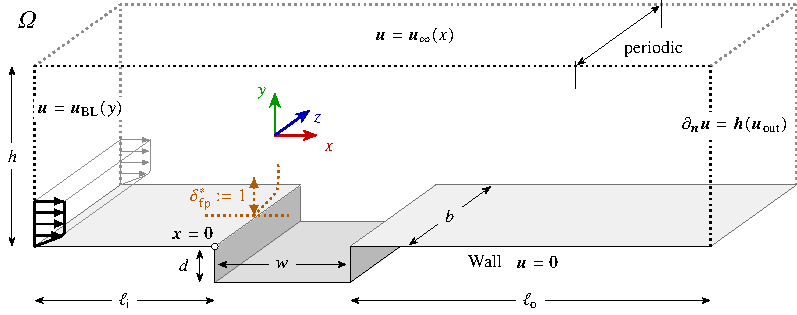
\includegraphics[width=\linewidth]{Images/domainBaseflow3D.pdf}
	\end{figure}
	\vspace{-0.3cm}
	\begin{itemize}
		\item (for the moment) Incompressible Navier--Stokes\pause
		\item $\Rey = u_\infty\dstar/\nu\in[800,3000]$ (mostly $\Rey=1000$), $w\in[0,130]$, $d\in[0,4]$.\pause
		\item \texttt{Nektar++}: spectral/$hp$ elements ($p=5$) in $(x,y)$ + Fourier in $z$ ($\sim4\times10^6$ dof in 3D).
	\end{itemize}
\end{frame}

%======================================================================
\section{Global stability analysis}
\begin{frame}{Step 1: base flows}
	\begin{itemize}
		\item Aim: \textbf{stability} of the laminar flow over the gap.
		\item First step: steady base flow $\vf{U}(x,y)$ from nonlinear DNS.
	\end{itemize}
	\begin{figure}
		\centering
		\begin{subfigure}{0.32\linewidth}
			\centering
			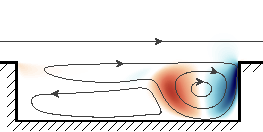
\includegraphics[width=\linewidth]{Images/gapd4_w15.pdf}
			\caption*{$w=15$, $d=4$ (open)}
		\end{subfigure}
		\begin{subfigure}{0.32\linewidth}
			\centering
			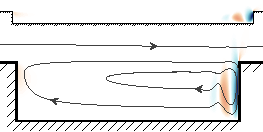
\includegraphics[width=\linewidth]{Images/gapd1.5_w30.pdf}
			\caption*{$w=30$, $d=1.5$}
		\end{subfigure}
		\begin{subfigure}{0.32\linewidth}
			\centering
			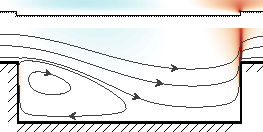
\includegraphics[width=\linewidth]{Images/gapd1_w60.pdf}
			\caption*{$w=60$, $d=1$ (closed)}
		\end{subfigure}\\[6pt]
		
\includegraphics[width=0.85\linewidth]{Images/colorbar_equilibriumBig.pdf}
	\end{figure}
	\pause
	\begin{itemize}
		\item \textbf{Narrow, deep} gaps: a recirculation vortex below a shear layer spanning the gap.
		\item \textbf{Wide, shallow} gaps: the shear layer reattaches, locally like a BFS followed by an FFS.
	\end{itemize}
\end{frame}

\begin{frame}{Step 2: linear stability of the base flow}
	\begin{itemize}
		\setlength\itemsep{0.8em}
		\item Linearise around $\vf{U}$, $\vf{u}=\vf{U}+\vf{u}'$, and look for eigenmodes
		      $$\vf{u}' = \hat{\vf{u}}(x,y)\,\mathrm{e}^{\ii\beta z}\,\mathrm{e}^{\lambda t}.$$\pause
		\item Track the \textbf{leading eigenvalue} for spanwise-uniform ($\beta=0$) and spanwise-varying ($\beta_n=2\pi n/b$, $n\geq1$) perturbations:
		      $$\sigma_\text{2D}(w,d) = \max_\lambda \operatorname{Re}\lambda\big|_{\beta=0}, \qquad \sigma_\text{3D}(w,d) = \max_{n\geq1}\, \max_\lambda \operatorname{Re}\lambda\big|_{\beta_n}.$$\pause
		\item The \textbf{neutral stability boundaries} in the $(w,d)$ plane are where $\sigma_\text{2D}$ and $\sigma_\text{3D}$ are zero.
	\end{itemize}
\end{frame}

\begin{frame}{2D and 3D stability boundaries vs experiment}
	\centering
	\begin{tikzpicture}[trim left=-10pt, trim right=\linewidth] % 3D mode may stick into the left margin
		% step 1: map without the zoom; step 2 on: with it (same geometry, see Images/src/stabCurveInsetSteps.py)
		\node[anchor=south west, inner sep=0] (stab) at (0,0) {\alt<1>{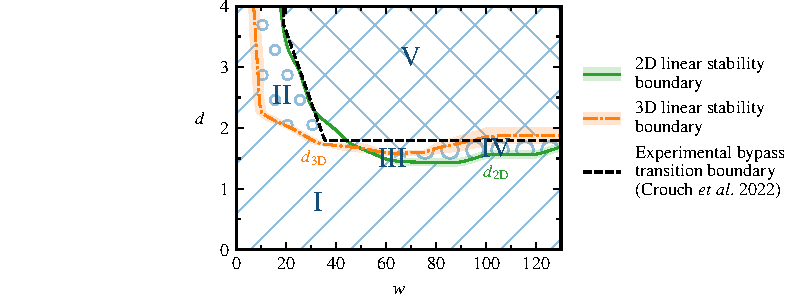
\includegraphics[width=\linewidth]{Images/stabCurveStep1.pdf}}{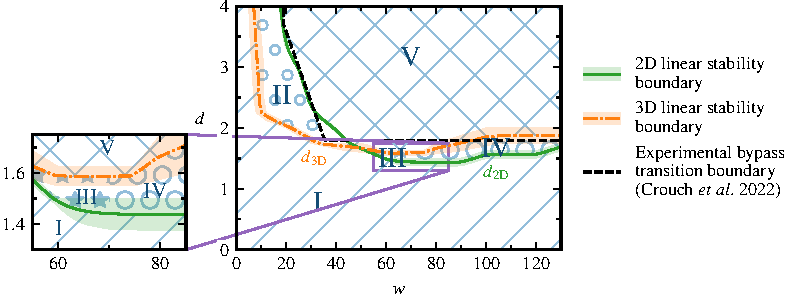
\includegraphics[width=\linewidth]{Images/stabCurveStep2.pdf}}};
		\begin{scope}[x={(stab.south east)}, y={(stab.north west)}]
			\node[anchor=north west, text width=0.44\linewidth, font=\footnotesize, inner sep=0] at (0.56,-0.04) {%
				\begin{itemize}
					\item \textcolor{mplgreen}{\bfseries\boldmath Green: $\sigma_\text{2D}=0$}\\ \textcolor{mplorange}{\bfseries\boldmath Orange: $\sigma_\text{3D}=0$}
					\item Deep gaps: \textbf{3D} first\\
					      Shallow gaps: \textbf{2D} first
					\item Experimental bypass boundary follows the \textbf{upper envelope} $\max\{d_\text{2D}, d_\text{3D}\}$.
				\end{itemize}};
			% 3D mode of (w,d)=(19,4), marker placed inside region II along w/d = 19/4
			\begin{scope}[visible on=<3->]
				\coordinate (pt3d) at (0.3435,0.8161);
				\node[anchor=north, inner sep=1pt] (m3d) at (0.10,-0.06) {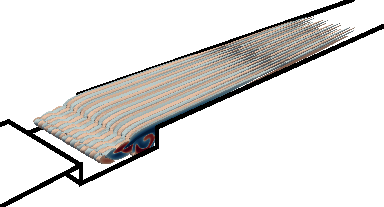
\includegraphics[width=0.32\linewidth]{Images/mode_d4w19_3dmode.pdf}};
				\node[anchor=north, inner sep=1pt, font=\scriptsize, align=center] at (m3d.south) {3D mode:\\\textbf{centrifugal}\\ \textbf{instability
					}};
				\draw[customcolor, thin] (pt3d) -- (m3d.north);
				\fill[customcolor] (pt3d) circle (1.5pt);
			\end{scope}
			% 2D mode of (w,d)=(19,4), marker exactly at (19,4)
			\begin{scope}[visible on=<4->]
				\coordinate (pt2d) at ({(314.5+25*433/130)/1063},{(64+81.25*3.5)/397});
				\node[anchor=north, inner sep=1pt] (m2d) at (0.41,-0.06) {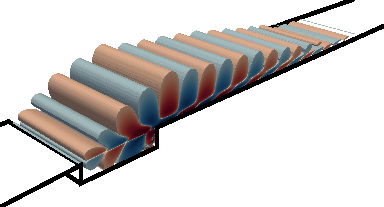
\includegraphics[width=0.32\linewidth]{Images/mode_d4w19_2dmode.pdf}};
				\node[anchor=north, inner sep=1pt, font=\scriptsize, align=center] at (m2d.south) {2D mode:\\\textbf{Rossiter-type}\\ \textbf{oscillation}};
				\draw[customcolor, thin] (pt2d) -- (m2d.north);
				\fill[customcolor] (pt2d) circle (1.5pt);
			\end{scope}
		\end{scope}
	\end{tikzpicture}
\end{frame}

%======================================================================
\section{Two-dimensional dynamics}
\begin{frame}{Region I: exciting TS waves}
	\begin{columns}[c]
		\begin{column}{0.45\linewidth}
			\small
			\begin{itemize}
				\setlength\itemsep{0.3em}
				\item TS waves are 2D, so we start with the \textbf{2D problem}.
				\item Region I: stable equilibrium, so we can linearise around it.\pause
				\item Divergence-free body force upstream, driven by Gaussian white noise.
				\item Measure the amplitude
				      $$A(x)^2 = \int \langle u'^2+v'^2\rangle_{\mathcal{T}}\,\dd{y}$$
				      and $n(x) = \log\left(A(x)/A(x_0)\right)$.
			\end{itemize}
		\end{column}
		\begin{column}{0.55\linewidth}
			\begin{figure}
				\centering
				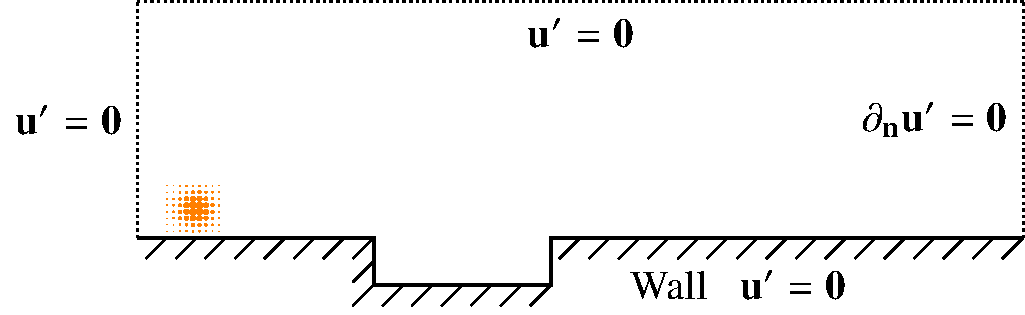
\includegraphics[width=\linewidth]{Images/domainPert.pdf}
			\end{figure}
		\end{column}
	\end{columns}
\end{frame}

\begin{frame}{$n$-factor curves: global vs local analysis}
	\begin{columns}[T]
		\begin{column}{0.49\linewidth}
			\centering
			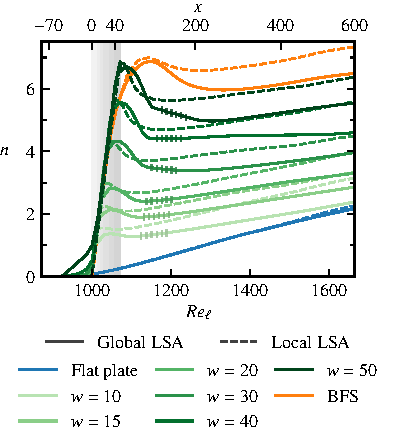
\includegraphics[height=6.6cm]{Images/nfactorCurvesLocald1.5.pdf}\\
			{\small Simulations, fixed $d=1.5$}
		\end{column}\pause
		\begin{column}{0.49\linewidth}
			\centering
			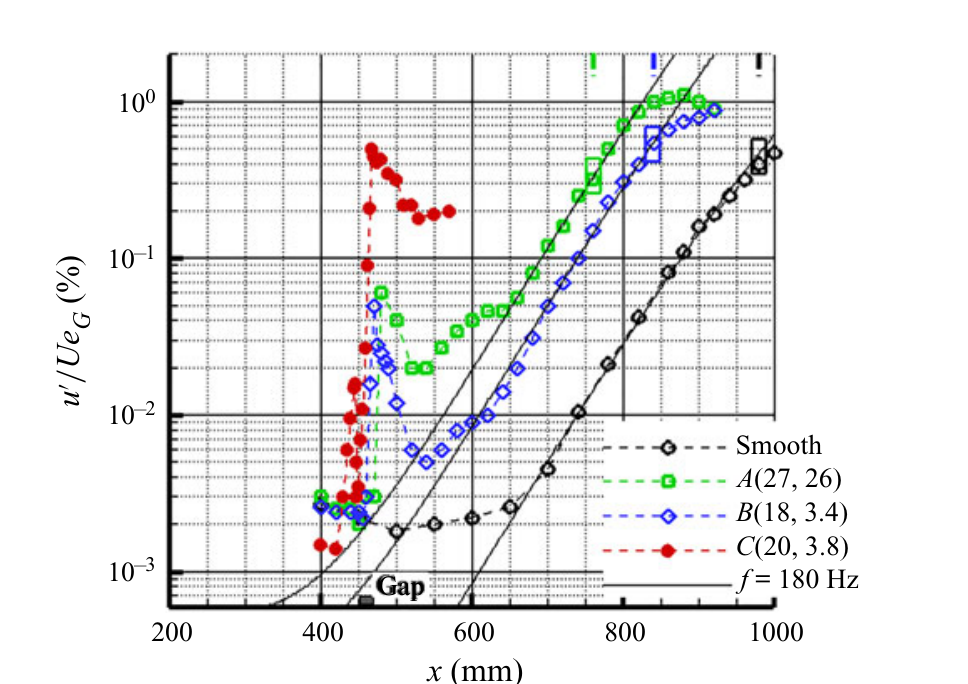
\includegraphics[width=0.9\linewidth]{Images/jeffAmplitude.png}\\
			{\small Experiments, Crouch \emph{et al.} (2022)}
			\footnotesize
		\end{column}
	\end{columns}
\end{frame}

\begin{frame}{Why that shape of the $n$ curves? Local LSA}
	\begin{columns}[c]
		\begin{column}{0.55\linewidth}
			\centering
			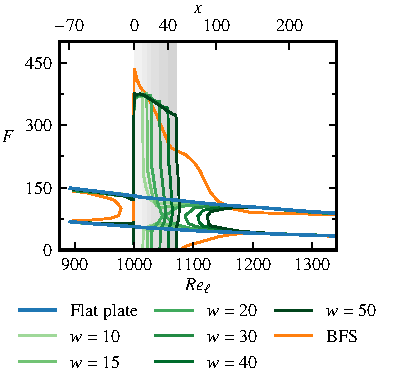
\includegraphics[width=\linewidth]{Images/neutralCurvesLocald1.5.pdf}\\
			{\small fixed $d=1.5$}
		\end{column}\pause
		\begin{column}{0.43\linewidth}
			\small
			\begin{itemize}
				\setlength\itemsep{0.5em}
				\item Over the gap, the shear layer destabilises a much broader range of frequencies.
				\item For \textbf{wide gaps} a locally stable region downstream the gap causes the drop in $n$.
			\end{itemize}
		\end{column}
	\end{columns}
\end{frame}

\begin{frame}{Definition $\Delta N$ vs $\Delta n$}
	\begin{columns}[c]
		\begin{column}{0.45\linewidth}
			\begin{itemize}
				\setlength\itemsep{0.5em}
				\item \textbf{Experiment} ($\Delta N$): lower the threshold, using the smooth-wall curve only:
				      $$\Delta N = n_\text{flat}(x^\text{trans}_\text{flat}) - n_\text{flat}(x^\text{trans}_\text{gap}).$$
				\item<2-> \textbf{Simulation} ($\Delta n$): raise the amplification curve:
				      $$\Delta n = \frac{1}{|\mathcal{X}|}\int_\mathcal{X} \left(n_\text{gap} - n_\text{flat}\right)\dd{x}.$$
				\item<3-> Equivalent \emph{if the gap only amplifies} incoming waves.
			\end{itemize}
		\end{column}
		\begin{column}{0.54\linewidth}
			\begin{figure}
				\centering
				\visible<2->{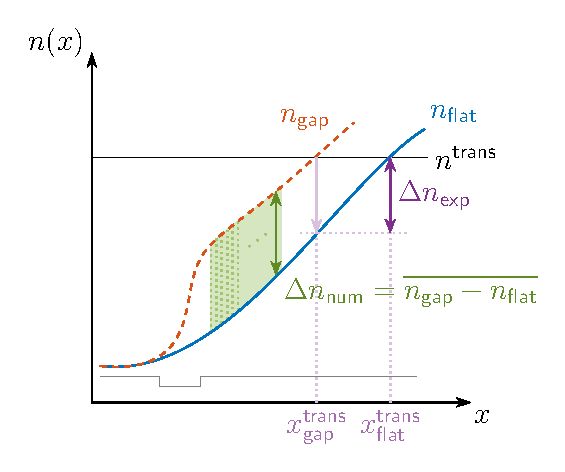
\includegraphics[width=1.08\linewidth]{Images/amplificationQualititiveNfactorLabels.pdf}}
			\end{figure}
		\end{column}
	\end{columns}
\end{frame}

\begin{frame}{Contours $\Delta N$ vs $\Delta n$}
	\begin{figure}
		\centering
		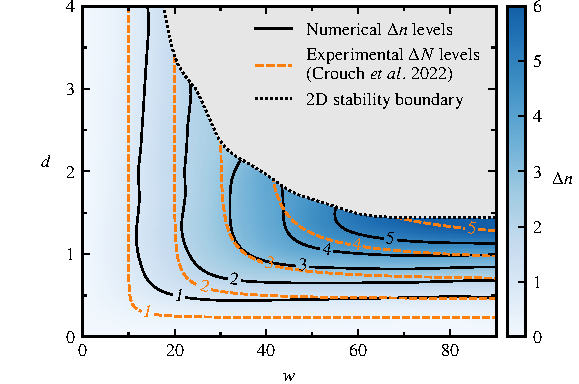
\includegraphics[width=0.9\linewidth]{Images/DeltaNcountour.pdf}
	\end{figure}
\end{frame}

\begin{frame}{Effect of Re on the stability boundary}
	\begin{figure}
		\centering
		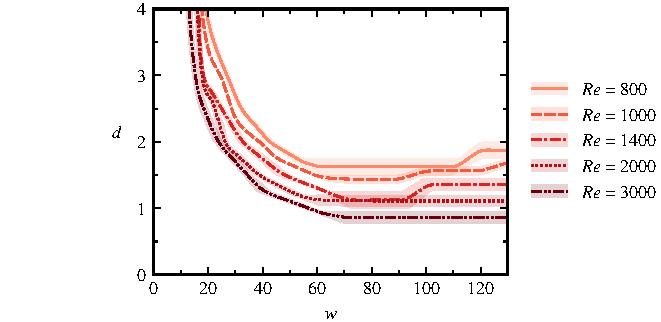
\includegraphics[width=0.95\linewidth]{Images/hopfBifReynolds.pdf}
	\end{figure}
	\takeaway{Increasing $\Rey$ moves the boundary to \textbf{smaller gaps}}
\end{frame}

\begin{frame}{Effects of Re on $\Delta n$ contours}
	\begin{columns}[c]
		\begin{column}{0.5\linewidth}
			\begin{figure}
				\centering
				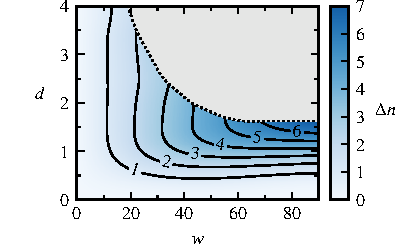
\includegraphics[width=\linewidth]{Images/DeltaNcountourOnlyNumericRe800.pdf}
				\caption*{$\Rey=800$}
			\end{figure}
		\end{column}
		\begin{column}{0.5\linewidth}
			\begin{figure}
				\centering
				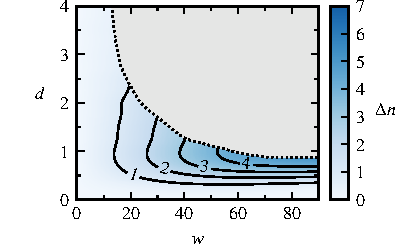
\includegraphics[width=\linewidth]{Images/DeltaNcountourOnlyNumericRe3000.pdf}
				\caption*{$\Rey=3000$}
			\end{figure}
		\end{column}
	\end{columns}\pause
	\begin{itemize}
		\item The stable region \textbf{shrinks} as $\Rey$ increases.
		      \pause
		\item Opposite trends:
		      \begin{itemize}
			      \item \textbf{narrow deep} gaps  amplify \emph{less} at higher $\Rey$
			      \item  \textbf{wide shallow} gaps amplify \emph{more} at higher $\Rey$
		      \end{itemize}
	\end{itemize}
\end{frame}

\begin{frame}{Why opposite trends?}
	% \vspace{0pt} makes [t] align the tops of the columns, not their first baselines
	\begin{columns}[t, onlytextwidth]\hspace{-0.4cm}
		\begin{column}{0.585\textwidth}
			\vspace{0pt}
			\vspace{-0.2cm}
			\begin{figure}
				\centering
				\begin{subfigure}{0.5\linewidth}
					\centering
					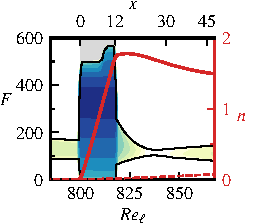
\includegraphics[width=\linewidth]{Images/localMapRe800_d4_w12.pdf}
					\caption*{\scriptsize $w=12,d=4$\\$\Rey=800$}
				\end{subfigure}%
				\begin{subfigure}{0.5\linewidth}
					\centering
					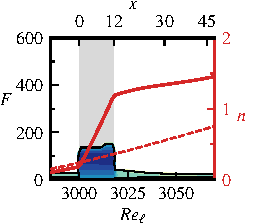
\includegraphics[width=\linewidth]{Images/localMapRe3000_d4_w12.pdf}
					\caption*{\scriptsize $w=12,d=4$\\$\Rey=3000$}
				\end{subfigure}\\[2pt]
				\begin{subfigure}{0.5\linewidth}
					\centering
					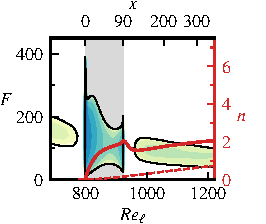
\includegraphics[width=\linewidth]{Images/localMapRe800_d0.5_w90.pdf}
					\caption*{\scriptsize $w=90,d=0.5$\\$\Rey=800$}
				\end{subfigure}%
				\begin{subfigure}{0.5\linewidth}
					\centering
					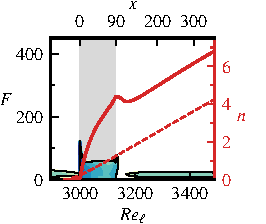
\includegraphics[width=\linewidth]{Images/localMapRe3000_d0.5_w90.pdf}
					\caption*{\scriptsize $w=90,d=0.5$\\$\Rey=3000$}
				\end{subfigure}
			\end{figure}
		\end{column}\hspace{-0.2cm}
		\begin{column}{0.13\textwidth}
			\vspace{1.5cm} % centred on the two rows of maps
			\makebox[\linewidth][l]{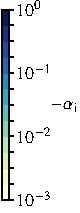
\includegraphics[height=3.6cm]{Images/localMapGrowthColorbarVertical.pdf}}
		\end{column}\hspace{-0.3cm}
		\begin{column}{0.37\textwidth}
			\vspace{0pt}
			\footnotesize
			\setlength\leftmargini{1em}
			\begin{itemize}
				\setlength\itemsep{0.5em}
				\item<2-> $\Delta n$ set by the unstable band \textbf{width}, its \textbf{growth rate} and the gap \textbf{length} $w$.
				\item<3-> Higher $\Rey$: narrower band, but stronger shear layer.
				      \begin{itemize}
					      \footnotesize
					      \item<3-> $w=12$: too short to profit $\Rightarrow\Delta n\downarrow$.
					      \item<3-> $w=90$: long enough to accumulate $\Rightarrow\Delta n\uparrow$.
				      \end{itemize}
			\end{itemize}
			\vspace{0.15cm}
			\uncover<4->{\takeaway{The \textbf{gap length} decides which effect wins.}}
		\end{column}
	\end{columns}
\end{frame}

\begin{frame}{Unsteady 2D dynamics}
	\begin{figure}
		\centering
		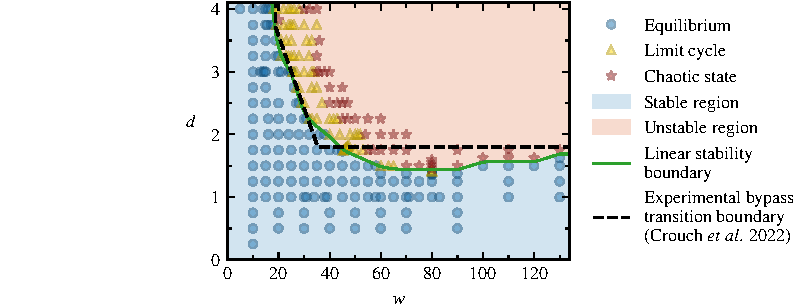
\includegraphics[width=\linewidth]{Images/inc2dStabilityCurveRe1000.pdf}
	\end{figure}
	\vspace{-0.3cm}\pause
	\begin{itemize}
		\item The linear stability boundary is \textbf{non-monotonic} in $w$: minimum near $(w,d)\approx(75,1.5)$, where the two edges interact most strongly.\pause
		\item The 2D modes set into a \textbf{limit cycle} via a supercritical Hopf bifurcation.\pause
		\item Further from the boundary: period doubling, then chaos (not investigated deeply).
	\end{itemize}
\end{frame}

\begin{frame}{Limit-cycle shape and amplitudes}
	\begin{figure}[ht]
		\centering
		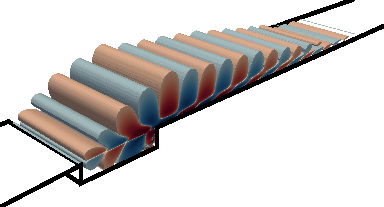
\includegraphics[width=4.2cm]{Images/mode_d4w19_2dmode.pdf}
	\end{figure}\pause
	\begin{figure}
		\centering
		% the pdf has ~21% blank margin on the left vs ~2% on the right: shift by half the difference
		\hspace*{-0.2\linewidth}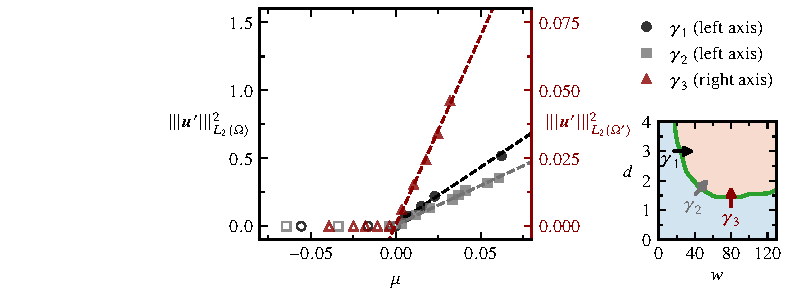
\includegraphics[width=\linewidth]{Images/hopfAmplitude.pdf}%
		% 2D mode of (w,d)=(19,4) in the empty upper-left corner (inline, so it takes no space)
	\end{figure}
	\pause
	\graybox{This confirms it is a \textbf{supercritical Hopf bifurcation}: $A^2\propto\mu$ along all paths.}
\end{frame}

\begin{frame}{Limit-cycle frequencies}
	\begin{figure}
		\centering
		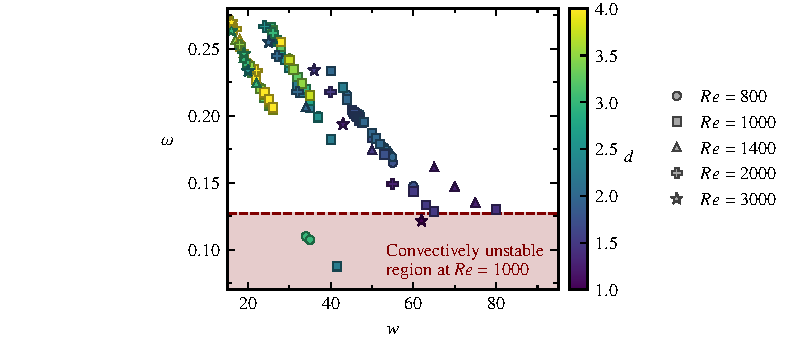
\includegraphics[width=\linewidth]{Images/freqUnstableMode.pdf}
	\end{figure}\pause
	\begin{itemize}
		\item Narrow gaps: discrete branches of cavity modes, well above the TS band.
		\item Wide gaps ($w\gtrsim65$): frequency drops towards the \textbf{TS band} (red), so the gap starts to act as a harmonic source for TS waves.
	\end{itemize}
\end{frame}

%======================================================================
\section{Three-dimensional dynamics and transition}
\begin{frame}{Region II: 3D mode saturates}
	\vspace{0.8cm} % clears the stability map in the top-right corner
	\begin{figure}
		\centering
		% step 1: stability map alone; step 2 on: field + connecting line
		\visible<2->{\tikz[remember picture, baseline] \node[inner sep=0pt] (etafig) {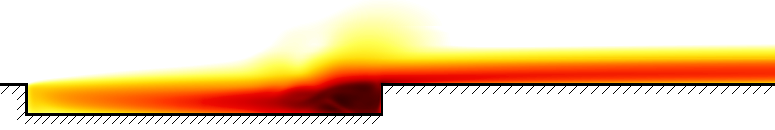
\includegraphics[width=\linewidth]{Images/gapd2_w24_3d_originalScaling.pdf}};}\\[4pt]
		\visible<2->{
\includegraphics[width=0.85\linewidth]{Images/colorbar_3d.pdf}}
	\end{figure}
	\begin{columns}[c]
		\begin{column}{0.32\linewidth}
			\centering
			\visible<3->{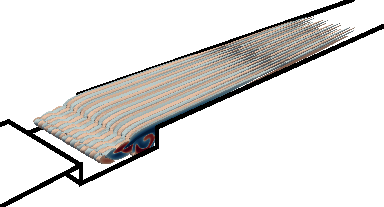
\includegraphics[width=1.1\linewidth]{Images/mode_d4w19_3dmode.pdf}}
		\end{column}
		\begin{column}{0.68\linewidth}
			\small
			\begin{itemize}
				\item<2-> $\eta=\sqrt{\langle|\vf{u}'|^2\rangle_{\mathcal{Z\times\mathcal{T}}}}$
				\item<3-> First linear exponential growth, then \textbf{saturation}. Distribution similar to the eigenmode.
				\item<4-> \textbf{No breakdown}: the downstream boundary layer remains laminar.
			\end{itemize}
		\end{column}
	\end{columns}
	\stabmap[3.8cm]{stabMapRegionII.pdf}
	% (w,d)=(24,2) on the map; axes fractions from Images/src/stabMapRegions.py
	\begin{tikzpicture}[remember picture, overlay]
		\begin{scope}[shift={(stabmap.south west)}, x={($(stabmap.south east)-(stabmap.south west)$)}, y={($(stabmap.north west)-(stabmap.south west)$)}]
			\coordinate (pt) at ({(0.9+5.5*28/130)/6.7}, {(0.8+4.125*2/4)/5.035});
		\end{scope}
		% ends at the mouth of the gap in the eta field
		\begin{scope}[shift={(etafig.south west)}, x={($(etafig.south east)-(etafig.south west)$)}, y={($(etafig.north west)-(etafig.south west)$)}]
			\coordinate (gapmouth) at (0.5, 0.7);
		\end{scope}
		\draw<2->[customcolor, thin] (pt) -- (gapmouth);
		\fill<2->[customcolor] (pt) circle (1.5pt);
	\end{tikzpicture}
\end{frame}

\begin{frame}{Regions III and IV: no bypass}
	\begin{columns}[c]
		\begin{column}{0.42\linewidth}
			\small
			\begin{itemize}
				\setlength\itemsep{0.5em}
				\item The 2D limit cycle is \textbf{stable to 3D perturbations}: no breakdown at the gap.
				\item<2-> What matters is its frequency relative to the TS band:
				      \begin{itemize}
					      \setlength\itemsep{0.3em}
					      \item<2-> \textbf{III}: \emph{above} the TS band $\Rightarrow$ damped downstream, \textbf{no transition}.
					      \item<2-> \textbf{IV}: \emph{below} its upper edge $\Rightarrow$ amplified, \textbf{triggers transition}.
				      \end{itemize}
			\end{itemize}
		\end{column}
		\begin{column}{0.58\linewidth}
			\vspace{1.2cm} % clears the stability map in the top-right corner
			\begin{figure}
				\centering
				\visible<2->{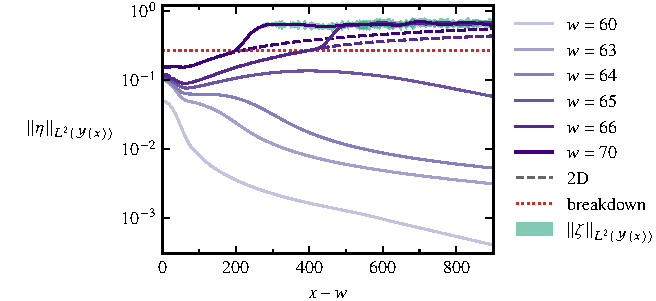
\includegraphics[width=\linewidth]{Images/L2POvsX.pdf}}
			\end{figure}
		\end{column}
	\end{columns}
	\stabmap[3.8cm]{stabMapRegionIII_IV.pdf}
\end{frame}

\begin{frame}{Region IV: TS-driven transition behind the gap}
	\vspace{2.3cm} % clears the stability map below the title
	\begin{figure}
		\centering
		% step 1: stability map alone; step 2 on: field + connecting line
		\visible<2->{\tikz[remember picture, baseline] \node[inner sep=0pt] (transfig) {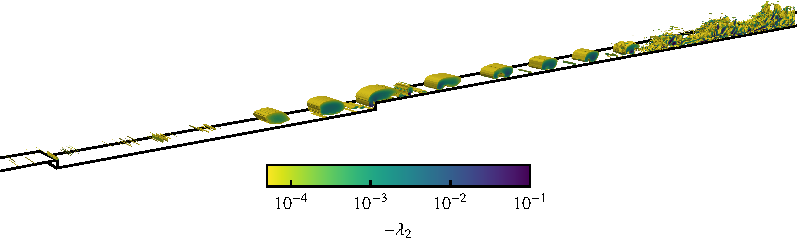
\includegraphics[width=\linewidth]{Images/trans_d1.5w80Lz5_3d_L2crit_31.pdf}};}
	\end{figure}
	\begin{itemize}
		\item<3-> The gap oscillation acts as a \textbf{self-sustained TS-wave source}.
		\item<4-> Breakdown happens \emph{downstream}, through the primary TS route.
	\end{itemize}
	% as \stabmap, but below the title, which is too long to share the corner
	% (w,d)=(80,1.5) on the map; axes fractions from Images/src/stabMapRegions.py
	\begin{tikzpicture}[remember picture, overlay]
		\node[anchor=north east, inner sep=0pt] (stabmap) at ([xshift=-0.05cm, yshift=-0.95cm]current page.north east)
		{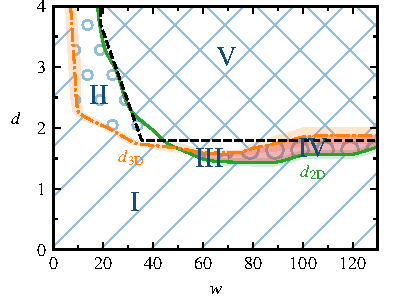
\includegraphics[width=3.4cm]{Images/stabMapRegionIII_IV.pdf}};
		\begin{scope}[shift={(stabmap.south west)}, x={($(stabmap.south east)-(stabmap.south west)$)}, y={($(stabmap.north west)-(stabmap.south west)$)}]
			\coordinate (pt) at ({(0.9+5.5*90/130)/6.7}, {(0.8+4.125*1.6/4)/5.035});
		\end{scope}
		% ends at the gap, at the upstream end of the 3D view
		\begin{scope}[shift={(transfig.south west)}, x={($(transfig.south east)-(transfig.south west)$)}, y={($(transfig.north west)-(transfig.south west)$)}]
			\coordinate (gap) at (0.5, 0.8);
		\end{scope}
		\draw<2->[customcolor, thin] (pt) -- (gap);
		\fill<2->[customcolor] (pt) circle (1.5pt);
	\end{tikzpicture}
\end{frame}
\begin{frame}{Region V: transition at the gap}
	\begin{figure}
		\vspace{1.1cm}
		\centering
		\begin{subfigure}{0.49\linewidth}
			\centering
			\visible<2->{%
				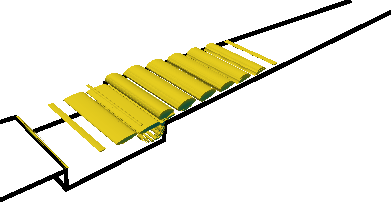
\includegraphics[width=\linewidth]{Images/trans_d4w19_3d_L2crit_10.pdf}
				\vspace{-1.2cm}
				\caption*{$t=1677$}
			}
		\end{subfigure}
		\begin{subfigure}{0.49\linewidth}
			\centering
			\visible<3->{%
				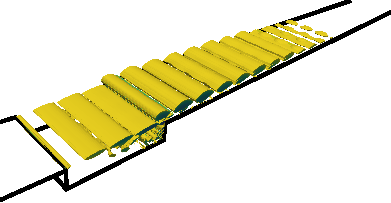
\includegraphics[width=\linewidth]{Images/trans_d4w19_3d_L2crit_12.pdf}
				\vspace{-1.2cm}
				\caption*{$t=2277$}
			}
		\end{subfigure}\\
		\vspace{-1.1cm}
		\begin{subfigure}{0.49\linewidth}
			\centering
			\visible<4->{%
				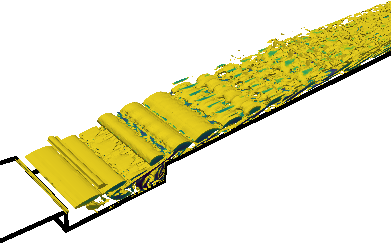
\includegraphics[width=\linewidth]{Images/trans_d4w19_3d_L2crit_14_big.pdf}
				\vspace{-1.2cm}
				\caption*{$t=2797$}
			}
		\end{subfigure}
		\begin{subfigure}{0.49\linewidth}
			\centering
			\visible<5->{%
				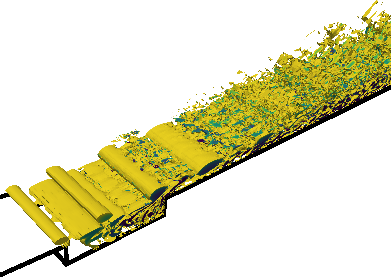
\includegraphics[width=\linewidth]{Images/trans_d4w19_3d_L2crit_17_big.pdf}
				\vspace{-1.2cm}
				\caption*{$t=3677$}
			}
		\end{subfigure}\\[2pt]
		\visible<2->{
\includegraphics[width=0.7\linewidth]{Images/trans_colorbarBig.pdf}}
	\end{figure}
	\stabmap{stabMapRegionV.pdf}
	% (w,d)=(40,3.4) on the map, joined to the slide at (50%, 80%) from the bottom left;
	% step 1: stability map alone; line from step 2 on
	\begin{tikzpicture}[remember picture, overlay]
		\begin{scope}[shift={(stabmap.south west)}, x={($(stabmap.south east)-(stabmap.south west)$)}, y={($(stabmap.north west)-(stabmap.south west)$)}]
			\coordinate (pt) at ({(0.9+5.5*40/130)/6.7}, {(0.8+4.125*3.4/4)/5.035});
		\end{scope}
		\draw<2->[customcolor, thin] ($(current page.south west)+(0.5\paperwidth,0.8\paperheight)$) -- (pt);
		\fill<2->[customcolor] (pt) circle (1.5pt);
	\end{tikzpicture}
\end{frame}

\begin{frame}{Why both instabilities are needed to bypass transition at the gap?}
	Quadratic nonlinearity: $(\beta_1,\omega_1)\times(\beta_2,\omega_2)\rightarrow(\beta_1\pm\beta_2,\omega_1\pm\omega_2)$\\\pause
	\begin{columns}[c]
		\begin{column}{0.48\linewidth}
			\small
			\begin{itemize}
				\setlength\itemsep{0.4em}
				\item 3D mode alone: forces only harmonics, the mean flow and slow 2D components, so it \textbf{saturates}.\pause
				\item $\omega_\text{2D}/\omega_\text{3D}\approx 9.6$: no resonant forcing of the 2D mode.\pause
				\item With the 2D oscillation present: sidebands $(\beta,\,\omega_\text{3D}\pm k\,\omega_\text{2D})$ spread energy across the spectrum, leading to \textbf{breakdown}.
			\end{itemize}
		\end{column}
		\begin{column}{0.5\linewidth}
			\begin{figure}
				\centering
				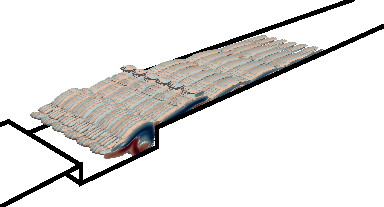
\includegraphics[width=\linewidth]{Images/mode_d4w19_3dFloquetmode.pdf}
				\caption*{\small Leading Floquet mode of the 2D limit cycle, $(19,4)$.}
			\end{figure}
		\end{column}
	\end{columns}
\end{frame}

\begin{frame}[t]{Summary of the incompressible picture}
	\vspace{0.45cm}
	\centering
	% Coordinates on 3d2dStabilityCurveRe1000NoInsetBlack.pdf as fractions of the image:
	% x = (70.5 + w*433/130)/819, y = (64 + 81.25*d)/397
	\begin{tikzpicture}[
		callout/.style={draw=customcolor, fill=customcolor!10, rounded corners=2pt, text width=3.4cm, align=left, font=\scriptsize, inner sep=3pt},
		link/.style={customcolor, thick, -{Stealth[length=4pt]}}]
		\node[anchor=south west, inner sep=0] (stab) at (0,0) {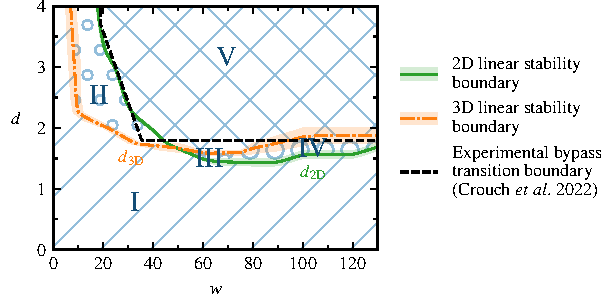
\includegraphics[width=0.62\linewidth]{Images/3d2dStabilityCurveRe1000NoInsetBlack.pdf}};
		\begin{scope}[x={(stab.south east)}, y={(stab.north west)}]
			\begin{scope}[visible on=<2->]
				\node[callout, anchor=north] (cI) at (0.1,-0.05) {\textbf{I} (stable): amplifier, $\Delta n$};
				\draw[link] (cI.north) -- (0.2081,0.2738);
			\end{scope}
			\begin{scope}[visible on=<3->]
				\node[callout, anchor=south west] (cII) at (-0.3,1.04) {\textbf{II} (3D unstable only): 3D mode saturates, BL stays laminar, still an amplifier.};
				\draw[link] (cII.south) -- (0.145,0.71);
			\end{scope}
			\begin{scope}[visible on=<4->]
				\node[callout, anchor=north] (cIII) at (0.75,-0.05) {\textbf{III} (2D unstable only): limit cycle, damped downstream.};
				\draw[link] (cIII.north) -- (0.38,0.42);
			\end{scope}
			\begin{scope}[visible on=<5->]
				\node[callout, anchor=south east] (cIV) at (1.3,1.04) {\textbf{IV} (2D unstable only): limit cycle seeds TS waves, transition downstream.};
				\draw[link] (cIV.south) -- (0.54,0.5603);
			\end{scope}
			\begin{scope}[visible on=<6->]
				\node[callout, anchor=south] (cV) at (0.5,1.04) {\textbf{V} (2D \& 3D unstable): transition at the gap (\textbf{bypass}).};
				\draw[link] (cV.south) -- (0.4,0.8775);
			\end{scope}
		\end{scope}
	\end{tikzpicture}
	\vspace{-0.1cm}
	\uncover<7->{\takeaway{Bypass transition at the gap occurs when the \textbf{2D limit cycle is itself unstable to 3D perturbations}.}}
\end{frame}

%======================================================================
\section{Compressibility}
\begin{frame}{Comments on compressibility (work in progress)}
	\begin{itemize}
		\setlength\itemsep{0.6em}
		\item The experiments of Crouch \textit{et~al.} are at $\Ma<0.1$. Cruise regime in commercial aircraft is at $\Ma\approx0.8$.
	\end{itemize}
\end{frame}

\begin{frame}{2D linear stability boundaries for different Ma}
	\begin{columns}[c]
		\begin{column}{0.58\linewidth}
			\begin{figure}
				\centering
				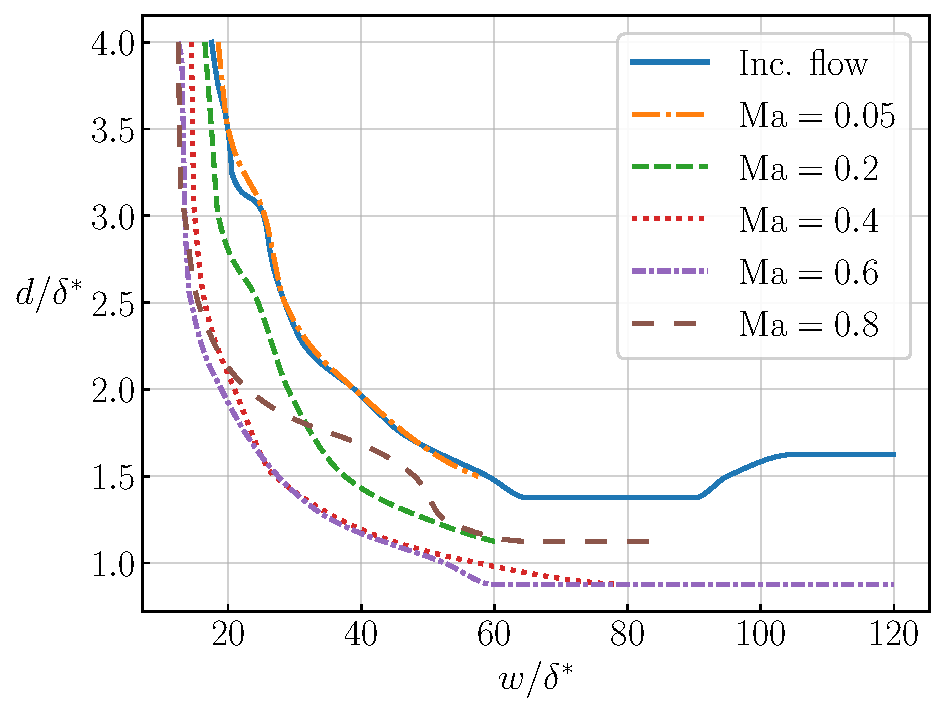
\includegraphics[width=\linewidth]{Images/Mabifurcations.pdf}
			\end{figure}\pause
		\end{column}
		\begin{column}{0.4\linewidth}
			\small
			\begin{itemize}
				\setlength\itemsep{0.4em}
				\item $\Ma=0.05$ recovers the incompressible boundary.\pause
				\item Compressibility is \textbf{destabilising}: the onset moves to smaller $w$ and $d$.\pause
				\item \textbf{Non-monotonic} in $\Ma$: $\Ma=0.8$ bifurcates later than $\Ma=0.6$ at intermediate depths. Why?\pause\ We don't know yet.
			\end{itemize}
		\end{column}
	\end{columns}
\end{frame}

\begin{frame}{Unstable mode at $d=2.5$}
	\begin{columns}[T]
		\begin{column}{0.49\linewidth}
			\centering
			$w=20$, $\Ma=0.6$\\
			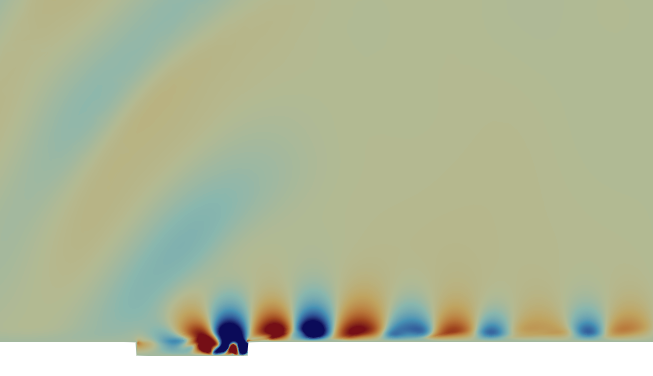
\includegraphics[width=\linewidth]{Images/d2.5_w20_Ma0.6.png}\\[0.2cm]\pause
			$w=20$, $\Ma=0.8$\\
			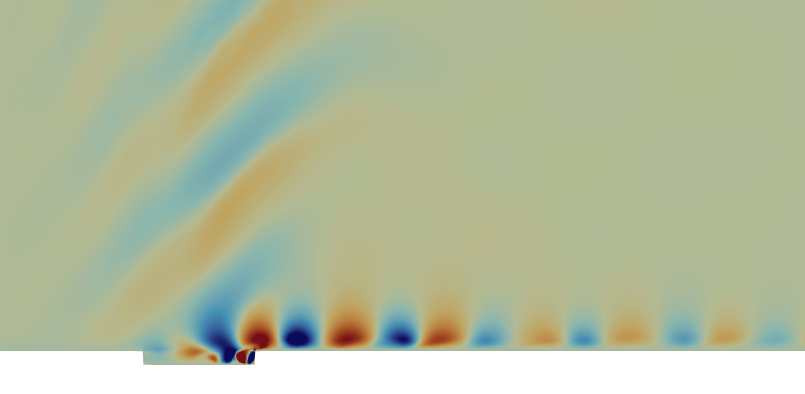
\includegraphics[width=\linewidth]{Images/d2.5_w20_Ma0.8.png}\pause
		\end{column}
		\begin{column}{0.49\linewidth}
			\centering
			$w=29$, incompressible\\
			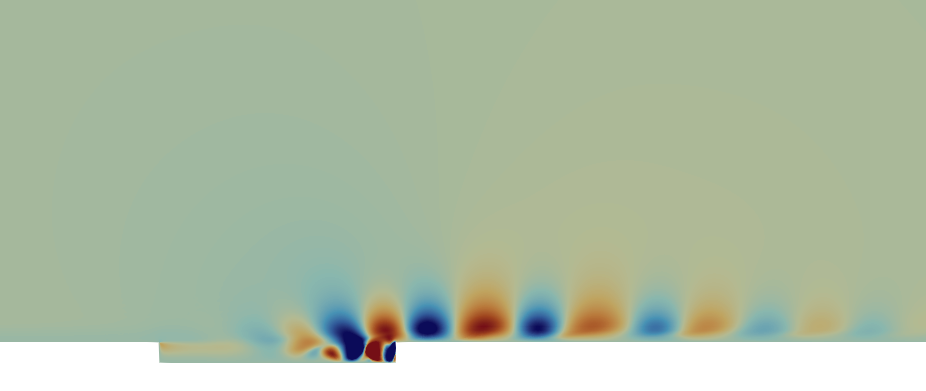
\includegraphics[width=\linewidth]{Images/d2.5_w29_inc.png}\\[0.3cm]\pause
			\begin{itemize}
				\small
				\item The same shear-layer mode becomes unstable at a \textbf{narrower} gap ($w=20$ vs $29$).\pause
				\item The Rossiter feedback loop is closed by \textbf{acoustic waves} travelling upstream from the downstream edge.
			\end{itemize}
		\end{column}
	\end{columns}
\end{frame}

%======================================================================
\section{Conclusions}
\begin{frame}{Conclusions}
	\begin{enumerate}
		\setlength\itemsep{0.6em}
		\item \textbf{Amplifier regime}: forced linear simulations reproduce the experimental $\Delta N$ map of Crouch \emph{et al.} The gap broadens the unstable TS band, and gap length decides the $\Rey$ trend.\pause
		\item \textbf{Oscillator regime}: the equilibrium is lost through a supercritical Hopf bifurcation (2D, shear layer) or a centrifugal 3D instability. The boundary moves to smaller gaps with $\Rey$.\pause
		\item \textbf{Transition at the gap} requires both instabilities (2D \& 3D). The 3D mode alone saturates.\pause
		\item \textbf{Compressibility} is destabilising and acoustically coupled, and non-monotonic in $\Ma$.
	\end{enumerate}
\end{frame}

\begin{frame}
	\centering
	{\Large\color{customcolor}\textbf{Thank you! Questions?}}\\[0.3cm]
	\small\texttt{v.ballester-ribo24@imperial.ac.uk}
\end{frame}

\end{document}
